% !TeX root = ../main.tex

\chapter{Theory}
\label{ch:theory}

\section{SVM}
A \acrfull{svm} is a machine learning algorithm which tries to separate binary-class training data. The \gls{svm} achieves this by searching for a hyperplane or a set of hyperplanes to separate the points of training data in a multidimensional space. There might be several possible hyperplanes that sufficiently separate the data but a \gls{svm} searches for the hyperplane with the biggest perpendicular distance between the hyperplane and the borders of both classes that should be separated. The space between the hyperplane and the closest of the training data points is defined as the margin. If the algorithm finds the maximal margin it has also found the optimal hyperplane. See figure \ref{fig:svmHyperplaneSeparation} for an example of possible hyperplane separations.

\begin{figure}[ht]
	\centering
	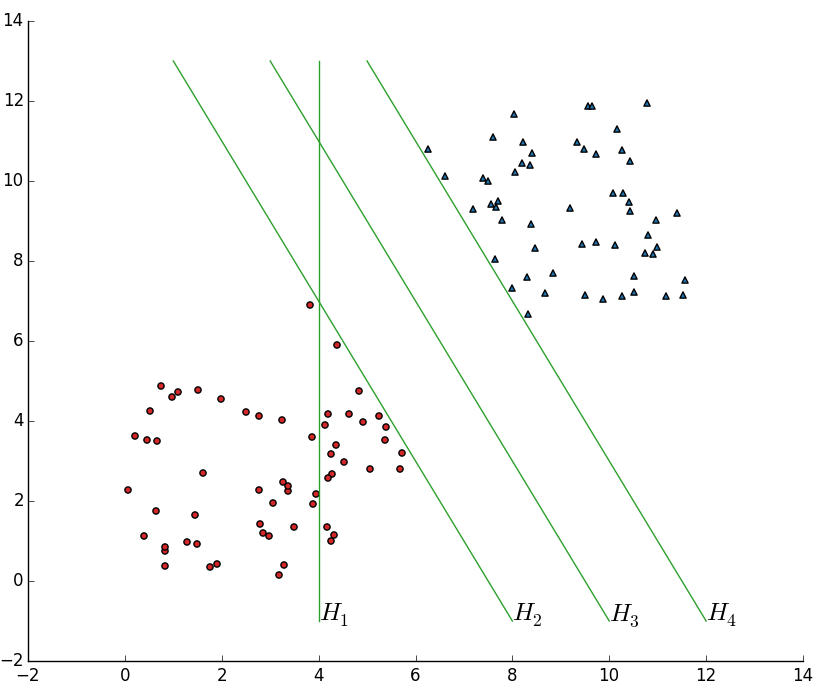
\includegraphics[scale=0.5]{figures/theorySVM_hyperplanes}
	\caption{Separation of two classes by hyperplanes in 2 dimensional space. $H_1$ does not separate, $H_2$ and $H_4$ separate but the margin is very slim, $H_3$ separates with a much better margin.}
	\label{fig:svmHyperplaneSeparation}
\end{figure}

\subsection*{Formal Definition}
Since a \Gls{svm} is a binary classifier a data point $x$ has to either belong into class A or class B. Let the training dataset of $n$ points be represented as $x_0,\dots,x_n$ and the target values be $y_0,\dots,y_n \in {-1,+1}$. The values of $y_n$ should be 
\begin{equation}
	y_i=
		\begin{cases}
		+1 & \text{if } x_i \in \text{class } {\color{red}A} \\
		-1 & \text{if } x_i \in \text{class } {\color{blue}B}
		\end{cases}.	
\end{equation}
The optimal hyperplane should separate all vectors $x_i$ with a value of $y_i=1$ {(class ${\color{red}A}$)} and those with a value of $y_i=-1$ {(class ${\color{blue}B}$)} so that the distance between those two groups is maximal \cite{Thome2012}. Let the hyperplane be
\begin{equation}
	D(x)=W \bullet x+b
\end{equation}

where $W$ is a vector normal to the hyperplane (see figure \ref{fig:svmHyperplaneDistance}) and $b$ is a bias term \cite{Boser1992}. $D(x)$ has to be calculated so that
\begin{equation}
	x \in 
	\begin{cases}
	\text{class } {\color{red}A} & \text{if } D(x) > 0 \\
	\text{class } {\color{blue}B} & \text{if } D(x) < 0
	\end{cases}	
\end{equation}
is true. The distance between a point $X$ and the hyperplane $D(x)$ is given as
\begin{equation}
\frac{D(X)}{\|W\|}
\end{equation}
which is illustrated in figure \ref{fig:svmHyperplaneDistance} \cite{Thome2012}. Assuming that the data is linear separable {(as in figure \ref{fig:svmHyperplaneSeparation})} we can then select two hyperplanes ${\color{red}D(x)>0}$ and ${\color{blue}D(x)<0}$ so that there are no points in between them and try to maximize the distance between those two hyperplanes {(in figure \ref{fig:svmHyperplaneSeparation} $H_2$ and $H_4$)} which is then given as 
\begin{equation}
\frac{2}{\|W\|}.
\end{equation}
To maximize the distance we must therefore minimize $\|W\|$ but with the constraint {(\ref{eq:svmHyperplaneCondition})} that no data gets between the two hyperplanes {(hard-margin classification)}. Both constraints
\begin{equation}
	\begin{split}
	x_i \bullet w+b \geq +1 \quad \text{if } {\color{red}y_i=+1}\\
	x_i \bullet w+b \leq -1 \quad \text{ if } {\color{blue}y_i=-1}
	\end{split}
\label{eq:svmHyperplaneCondition}
\end{equation}
can be combined to $y_i(x_i\bullet w + b)\geq 1\quad \forall i, i=1\dots n$. The solution for a maximum margin can therefore be found by solving
\begin{equation}
\begin{split}
\operatorname*{arg\,min}_{w, b}	\left\{\frac{1}{2}\|W\|^2\right\} \text{subject to} \\
y_i(x_i\bullet w + b)-1\geq 0 \quad \forall i, i=1\dots n	
\end{split}
\end{equation}
with the Lagrangian multiplier method \cite{Thome2012}. 

If the data is not linear separable we have to relax the constraints from \ref{eq:svmHyperplaneCondition} and allow some points in the margin {(soft-margin-classification)}. 

Classification of unknown data is now simply done through a calculation of the decision function $D(x)$
\begin{equation}
\text{prediction}
	\begin{cases}
	x \in \text{class } {\color{red}A} & \text{if } D(x) > 0 \\
	x \in \text{class } {\color{blue}B} & \text{if } \text{otherwise}
	\end{cases}	
\end{equation}

\begin{figure}[ht]
	\centering
	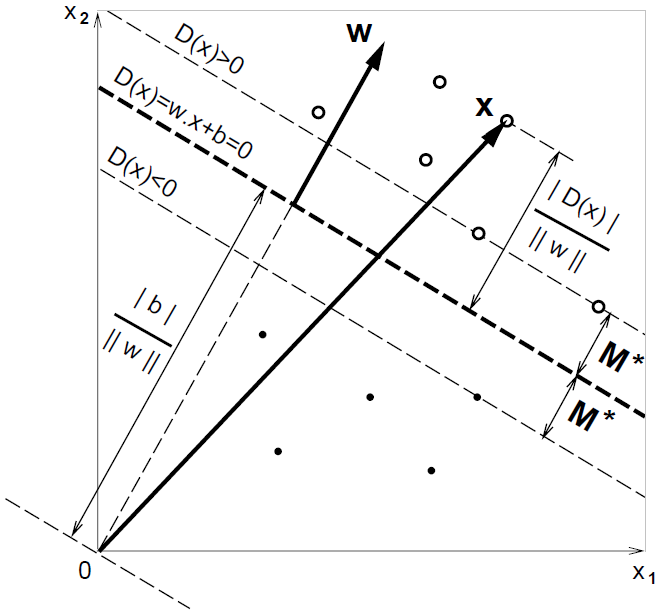
\includegraphics[scale=0.4]{figures/theorySVM_distanceToW}
	\caption{Visualization of optimal margin and hyperplane in 2 dimensional space. The distance of Point $X$ to $D(x)$ is $\frac{D(X)}{\|W\|}$. Source Bosner et al. \cite{Boser1992}.}
	\label{fig:svmHyperplaneDistance}
\end{figure}
\subsection*{Kernel Trick}
However, there are still cases where the data can not be separated by a linear function as shown in figure \ref{fig:svmKernelTrick}. In this case the data is mapped into another higher dimensional feature space {(Kernel trick)} so that it becomes linear separable again. The function that maps the data is called kernel. For evaluation in chapter \ref{ch:discussion} the following four kernels from OpenCV \cite{bradski2000opencv} and sklearn \cite{Pedregosa2011} were used:
\begin{itemize}
	\item Linear kernel: $k(x,y)=x*y$
	\item Polynomial kernel: $k(x,y)=(\gamma \left\langle x, y \right\rangle + coef_0)^\text{degree}$
	\item Radial basis function kernel: $k(x,y)=\exp(-\gamma ||x-y||^2)$
	\item Additive $\chi^2$ kernel: $ k(x,y)=-\sum \left[ (x-y)^2 / (x+y)\right] $
\end{itemize}
\begin{figure}
	\centering
	\subfloat[Data not separable]{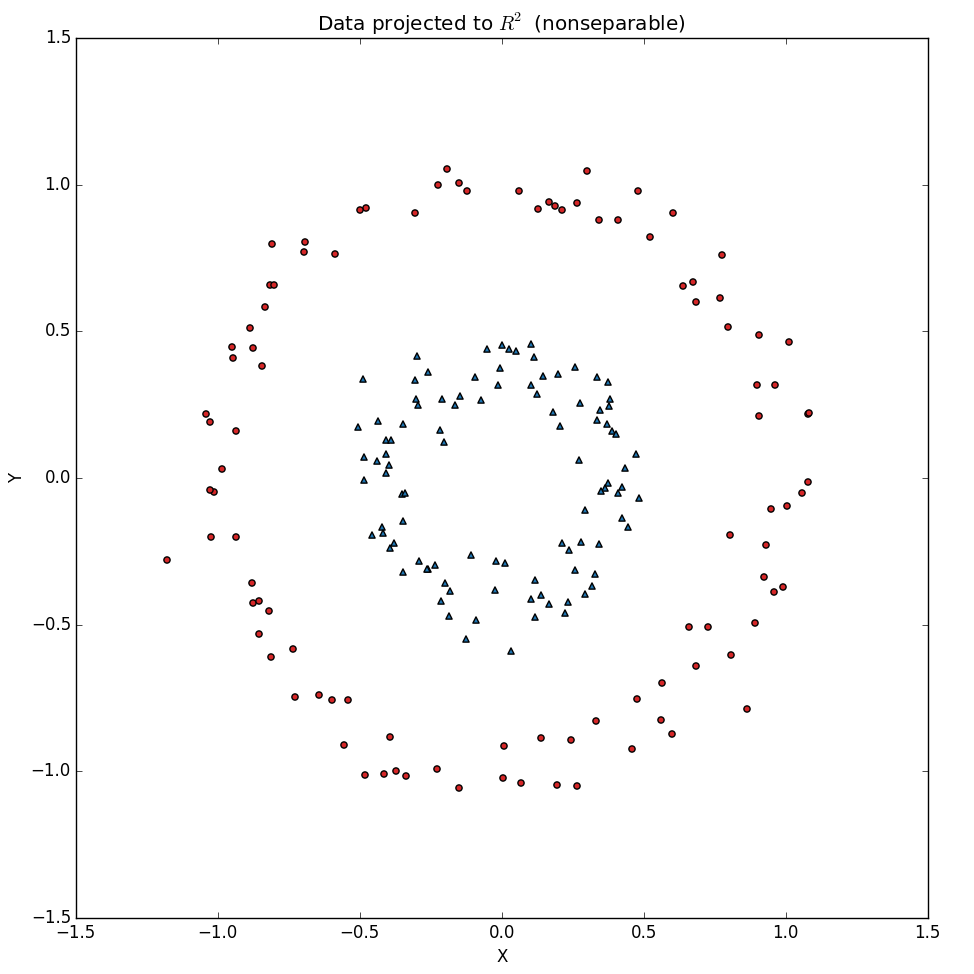
\includegraphics[width=55mm]{figures/theorySVM_kernelTrick1}}
	\subfloat[Data separable]{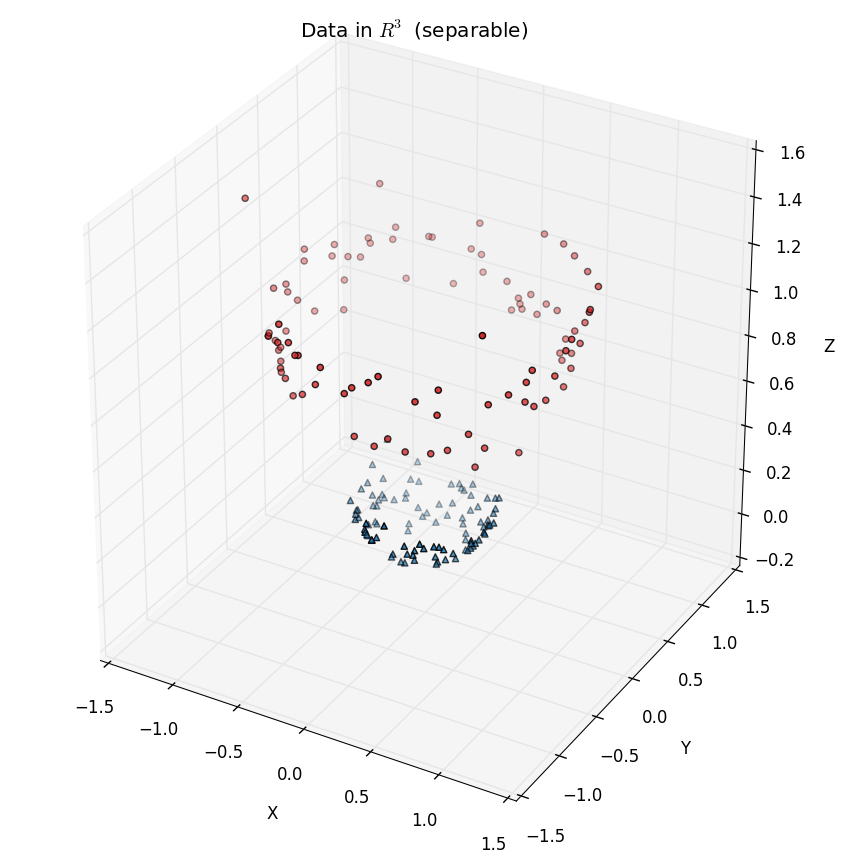
\includegraphics[width=55mm]{figures/theorySVM_kernelTrick2}}
	\subfloat[Data separable with hyperplane]{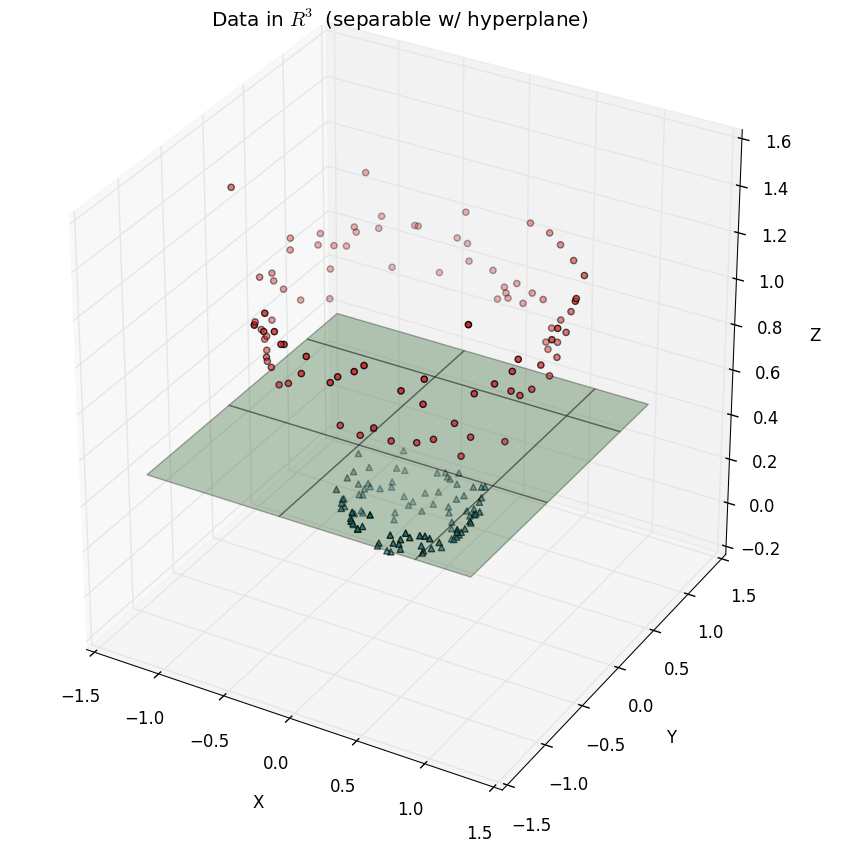
\includegraphics[width=55mm]{figures/theorySVM_kernelTrick3}}	
	\caption{Illustration of Kernel trick. Data in {(a)} is not separable but if the data gets mapped into a higher dimensional space {(b)} a linear hyperplane can be fitted {(c)}. Figures plotted with code adapted from \texttt{http://www.eric-kim.net/eric-kim-net/posts/1/kernel\_trick.html}}
	\label{fig:svmKernelTrick}
\end{figure}

\subsection*{Multiclass SVMs}
\label{subsec:svmMulticlass}
In case of a multiclass \gls{svm} problem the most popular approach is to use several different binary class \glspl{svm} instead of only one multiclass \gls{svm} \cite{Hsu2002, Duan2005, Thome2012}. There are two common solutions for the multiclass problem: One-VS-Rest and One-VS-One.

An One-VS-Rest multiclassifier with $n$ classes consists of $n$ distinct \glspl{svm}. Each \gls{svm} is trained on one of the classes as class A {(positive features)} and all other samples as class B {(negative features)}. Classification is done in a "winner-takes-it-all" fashion meaning that the \gls{svm} with the highest output function assigns the class label.

In the One-VS-One approach $n\frac{n-1}{2}$ \glspl{svm} are constructed. Each class is paired in a \gls{svm} with each other class. Classification is done in a "majority-vote" fashion so each \gls{svm} votes for its class and the class with the most votes is assigned as the class label.
\newpage
\section{K-Nearest Neighbors}
The \gls{knn} algorithm is a lazy classification algorithm which stores the complete training data in the learning phase \cite{Keller1985}. In the classification phase it searches for the $k$ points in the training data that are nearest to the point that should be classified. The label that gets the majority of votes from the $k$ closest points {(neighbors)} is the result of the classification. See figure \ref{fig:knn3} for a three class example and $k=3$. 

The most popular metric to get the distance between the neighbors is the Euclidean distance, however, the accuracy can greatly be improved by using a learned distance metric such as the Mahanalobis distance which tries to maximize the margin between classes \cite{Weinberger2005}. 

\begin{figure}[ht]
	\centering
	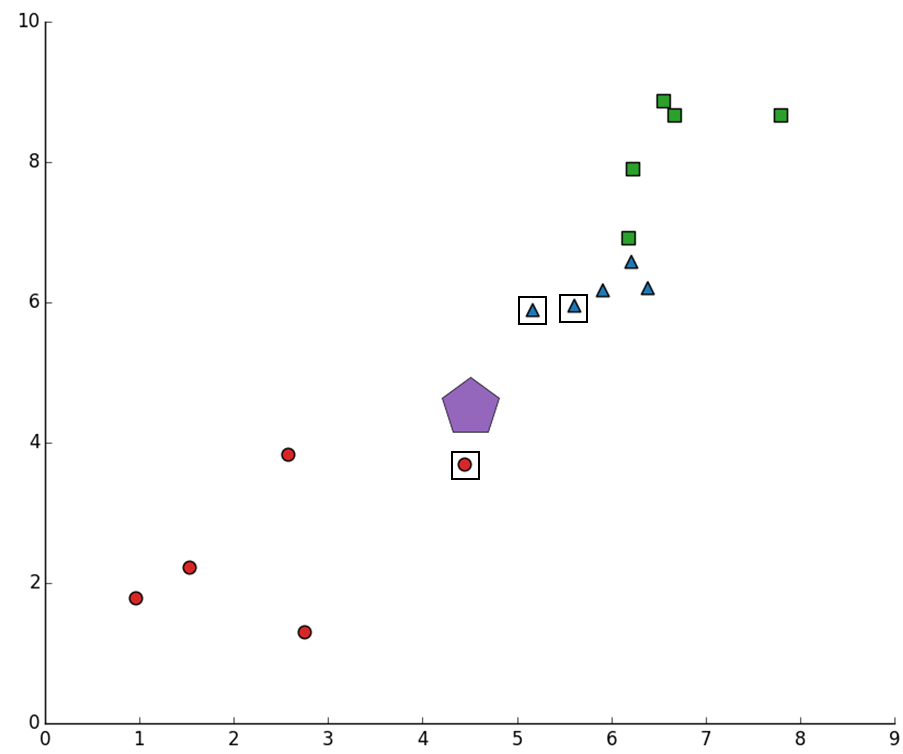
\includegraphics[scale=0.45]{figures/theoryKNN_3}
	\caption{Example for a knn classification with $k=3$. The three nearest elements to the purple pentagon {(point that should be classified)} are marked with a square. Since two of the three neighbors are triangles the new point should also be a triangle.}
	\label{fig:knn3}
\end{figure}

\section{Convolutional Neural Networks}
\begin{figure}[ht]
	\centering
	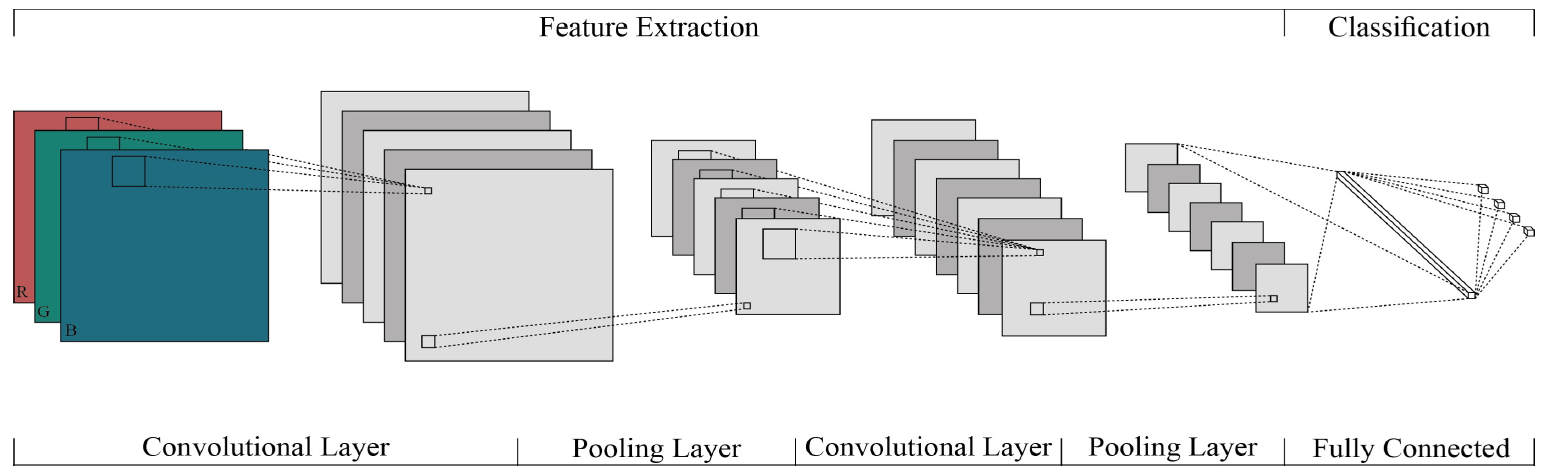
\includegraphics[scale=0.35]{figures/theoryCNN_model}
	\caption{Sample architecture of a \gls{cnn}. Source: Christodoulidis and Anthimopoulos \cite{Christodoulidis2015}}
	\label{fig:cnnModel}
\end{figure}
A \acrfull{cnn} is a multi-layer-feed-forward neural network that emulates the processes in the visual cortex by employing feature detection with small convolutional filters. \glspl{cnn} generally outperform other gradient based learning techniques \cite{LeCun1998} and are currently state-of-the-art \cite{Russakovsky2015} for image recognition.

\glspl{cnn} usually consist of a succession of trainable convolutional, dense and pooling layers. Normally, the first layers comprise of several convolutional and pooling layers for feature extraction. For the classifications of features extracted in the previous layers, the network has at least one dense layer of neurons before the last layer. The last layer is usually the output layer and for the standard classification task the number of neurons is equal to the number of classes to classify so that the output of a neuron is the probability of a specific class at the same time. Figure \ref{fig:cnnModel} shows an example of a \gls{cnn} architecture with two convolutional and pooling layers and a dense, fully connected layer before the output layer. 

\subsection*{Convolutional Layers}
\begin{figure}[ht]
	\centering
	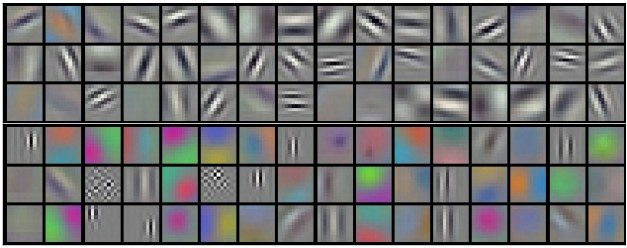
\includegraphics[scale=0.45]{figures/theoryCNN_filter}
	\caption{96 convolutional filters of size $3\times 11\times 11$ in the first layer. Filters trained on \gls{ilsvrc}-2010. Source: Krizhevsky et al. \cite{Krizhevsky2012}}
	\label{fig:cnnFilter}
\end{figure}
Convolutional layers contain multiple convolutional filters or kernels. They convolve the image to extract image features. Each filter convolves the output of the previous layer. In case of the first layer the filters operate directly on the input image. In later layers they collect more complex features from previous layers. Convolution happens by calculating the dot-product of the input matrix with the convolutional filter. Filters in \glspl{cnn} usually overlap which helps to get a better translation invariance since each pixel is convolved multiple times by the same filter. The main goal of convolution in \glspl{cnn} is to get distinctive image features. These convolutional filters are not handcrafted like filters in typical feature detectors. They learn the best filters by learning large quantities of data and change over the time and are ultimately able to extract features that are characteristic for the problem. Often, these kernels extract simple features like horizontal, vertical or diagonal edges {(figure \ref{fig:cnnFilter})}. For food, prominent first layer kernels typically include many color kernels that specialize in extracting a range of similar colors \cite{Christodoulidis2015}. The basic idea behind convolutional filters is that many features like edges or corners appear in multiple locations in images. By using the filters as a sliding window, one filter is able to detect the feature in any position.  

Therefore, the main befit of using convolutional filters is the reduction of learnable weights. Filters are very small {(7x7 as the maximum size for a current \gls{cnn} \cite{Szegedy2014})} but are applied on the whole image in a sliding window approach. This means that a single convolutional filter shares weights for the image which significantly improves learning because it reduces the number of parameters to learn \cite{LeCun1998}. GoogLeNet, a 22-layer \gls{cnn}, uses \gls{rgb} input images with a size of 224x224 \cite{Szegedy2014}. A normal Neural Net without convolutions would not be able to handle this input size.

\subsection*{Pooling Layers}
Once a feature is detected the exact position becomes less important. Only the spatial relation to other features remains valuable. Knowing the exact position of a feature may even be harmful for generalization because the model becomes less invariant to position \cite{LeCun1998}. One way to solve this problem and reduce the number of weights to learn is subsampling. In \glspl{cnn} this normally occurs in pooling layers. Currently, the most common pooling layer type is max-pooling. This filter basically divides the input into $z\times z$ blocks and extracts the maximum value of each block. A popular max-pooling layer instance is a $z=2$, stride $s=2$ layer. This layer downsamples the input by two. Recently, overlapping max-pooling layers have become popular \cite{Szegedy2014}. They do not downsample as much as non-overlapping pooling layers {(in fact $z=3$ and $s=2$ outputs the same dimensions as the input)} but they seem to slightly decrease the error \cite{Krizhevsky2012}.

\subsection*{Overfitting and Dropout}
\label{subsec:overfittingDropout}
Although \glspl{cnn} need fewer parameters to train high dimensional inputs than conventional neural nets, they also have the tendency to overfitt like conventional nets do. Overfitting is a common problem in machine learning that occurs if models are very complex. An overfitted model is optimized across the training data and describes or "fits" this data so well that it can not explain unseen data \cite{Falkenauer1998}. Figure \ref{fig:overfittingNet}a shows an overifitting neural network. After epoch 80 the error on the training set continues to decrease but the error on the validation set stops to decrease which means that although the net gets better at predicting the training data it gets worse for predicting unseen data.

Dropout is a novel way for neural nets to reduce the problem of overfitting by randomly dropping out nodes from the model. This forces the net to generalize better \cite{Srivastava2014}.

\subsection*{Learning Rate and Momentum}
\label{subsec:learningMomentum}
Neural networks try to find the global minimum of their cost function by adjusting the network weights. If there is only one minimum this is fairly easy as the network only has to adjust the weights towards the downward gradient. Real world scenarios, however, are much more complex and include many local minima as well. 

Learning rate and momentum are measurements of how weights are adjusted in backpropagation in search of the global minima. The learning rate denotes the magnitude of the weight change. That means that networks with a high learning rate advance faster along the gradient. Momentum is a term that multiplies a fraction of the previous weight update to the weight adjustment. By applying momentum, the steps the network takes on the gradient towards the minimum get bigger with each iteration. This helps to increase the speed of learning and may also prevent the network from getting stuck on local minima and saddle points because of the "momentum" the network simply "steps over" these points.

\section{Feature detectors and descriptors}
A common approach in image classification is the use of feature detectors and feature descriptors. A feature detector detects interest points or keypoints in images. Ideally those keypoints are invariant to image transformations like rotation, scale or illumination changes so that the points can be found even if the image is rotated or taken from another perspective. In most cases, keypoints are corners, as corners can be localized quite easily. Knowing that a corner exists, however, does not help much with recognition. An algorithm also needs to describe the characteristics of an interest point so that it is possible to compare different interest points. The part of describing a keypoint is done by keypoint descriptors.

\subsection[HOG]{Histograms of Oriented Gradients (HOG)}
\begin{figure}
	\centering
	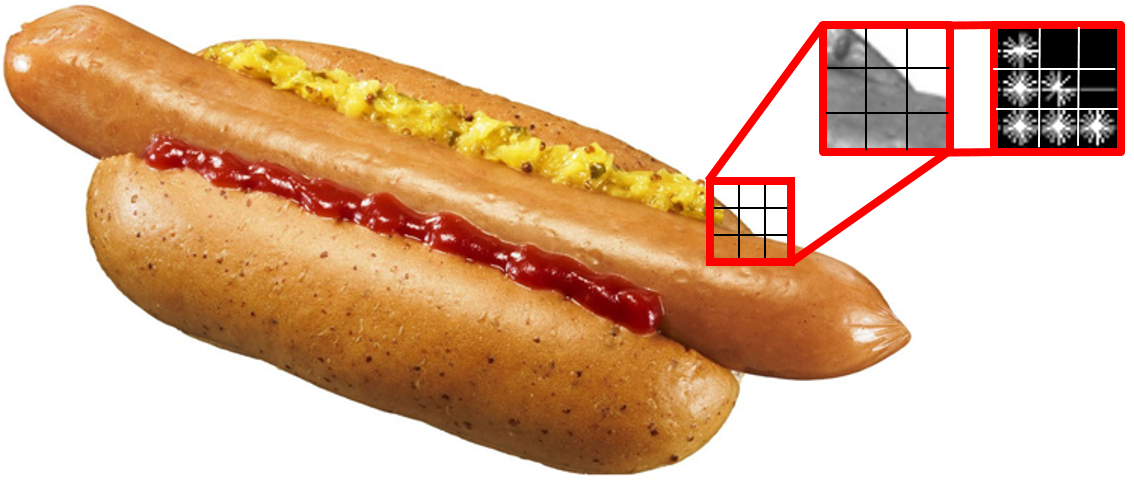
\includegraphics[scale=0.45]{data/images/theory/theoryHOG_VisualizationGradients}
	\caption{Visualization of HOG descriptor.}
	\label{fig:hogVisualization}
\end{figure}

\acrfull{hog} is a popular image descriptor for human detection, developed by Dalal and Triggs in 2005 \cite{Dalal2005}. The algorithm makes use of small contrast changes by describing the distribution of local gradients. This approach is believed to be based on biological processes of neurons in the primary visual cortex \cite{Lowe2004}.

The first step is to divide the image into small blocks with a size of 16x16 pixels and a 50\% overlap for better results. Each block is then subdivided by four 8x8 pixel cells. For each of these cells, gradient intensities are computed by applying the 1-D centered point derivative convolution mask horizontally and vertically:
\begin{equation}
	D_x=
	\begin{bmatrix}
	-1 & 0 & 1
	\end{bmatrix} 
	\quad
	D_y=
	\begin{bmatrix}
	-1 \\ 0 \\ 1
	\end{bmatrix} 
\end{equation}   
The magnitude of the gradients is
\begin{equation}
	m=\sqrt{(I\ast D_x)^2+(I\ast D_y)^2}
\end{equation}
where $I$ is the image cell and the gradient orientation is given as
\begin{equation}
	\theta = \arctan \left[\ \frac{(I\ast D_y)}{(I\ast D_x)}\right]\text{.}
\end{equation}
To achieve a better illumination invariance against shadowing, it is useful to contrast-normalize each cell. 

To get a feature vector for each cell, a 9-bin histogram of the gradient orientations {(0\degree - 180\degree)} is calculated. The gradient orientations $\theta$ are then scaled by the corresponding magnitude $m$. Figure \ref{fig:hogVisualization} shows a visualization of gradient histograms. The gradient histogram in the center row on the right, is a single horizontal line meaning that the gradients in this cell are all horizontal which is logical because the original image in this cell is a horizontal edge.

To get the feature vector for the whole image all histograms are concatenated to form a large gradient histogram.

\gls{hog} is not rotation invariant which does not matter for human detection as humans tend to always have the same upright orientation. However, for food, rotation invariance is quite important.

\subsection[LBP]{Local Binary Pattern (LBP)}
\begin{figure}[ht]
	\centering
	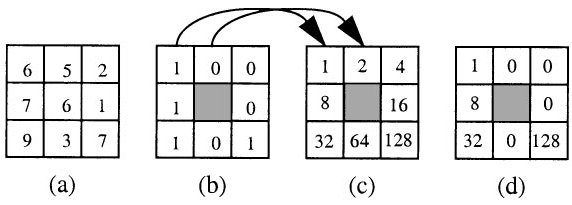
\includegraphics[width=\linewidth]{figures/theoryLBP_coding}
	\caption{Example for a LBP coding of the center pixel with value 6 (a). The neighboring pixels are thresholded against the center value (b) and multiplied by values in (c) with the result in (d). Source: Ojala et al. \cite{Ojala1999}}
	\label{fig:lbpCoding}
\end{figure}
\acrfull{lbp} is a simple texture descriptor which was originally proposed by Ojala et al. in 1994 \cite{Ojala1994}. For the calculation of the \gls{lbp} descriptor the 8 neighbors in a 3x3 block for each pixel are taken into account {(fig \ref{fig:lbpCoding}a)}. The neighbors of the center pixel are then thresholded by comparing the value {(grayscale intensity)} of the pixel in the center to the intensities of the neighboring pixels. Pixels with a higher or equal value are getting labeled as "1" and "0" otherwise {(fig \ref{fig:lbpCoding}b)}. Each position in the 3x3 block is then assigned a weight of $2^n$ {(fig \ref{fig:lbpCoding}c)} where $n$ is ascending from left-to-right, top-to-bottom. In recent publications these weights are labeled clockwise ascending. The binary values are than multiplied by the corresponding weights {(fig \ref{fig:lbpCoding}d)}. The values are then summed up and assigned as the new value for this "texture unit". The values can then be inserted into a histogram to form a 256-dim feature vector since there are 256 possible LBP values {($2^8=256$)}. Local binary patterns are invariant to grayscale changes because \gls{lbp} describes spatial texture structure but not contrast intensities \cite{Ojala1999}.  

In the following years \gls{lbp} has been adapted and extended with additional contrast information \cite{Ojala1999} or different neighborhood sizes to achieve rotation invariance with uniform \glspl{lbp} \cite{Ojala2002}.


\subsection[SIFT]{Scale invariant feature transform (SIFT)}
\label{subsec:sift}
\acrfull{sift} is a very popular local image feature detector, descriptor and matcher by Lowe from 1999 \cite{Lowe1999}. It is invariant to uniform image scaling, translation and rotation and partially invariant to affine distortions, 3D viewpoint and illumination changes. It is also invariant to noise, partial occlusion and clutter \cite{Lowe1999}. 

\subsubsection*{Keypoint detection}
%\begin{figure}
%	\centering
%	\begin{minipage}{.5\textwidth}
%		\centering
%		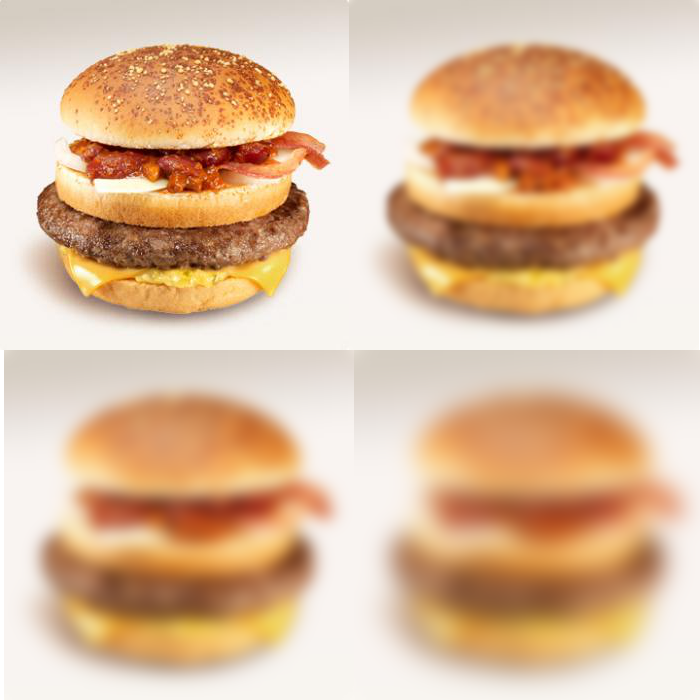
\includegraphics[width=0.45\linewidth]{data/images/theory/theorySIFT_gaussianScales}
%		\captionof{figure}{Image with different Gaussian scales.}
%		\label{fig:gaussianScales}
%	\end{minipage}%
%	\begin{minipage}{.5\textwidth}
%		\centering
%		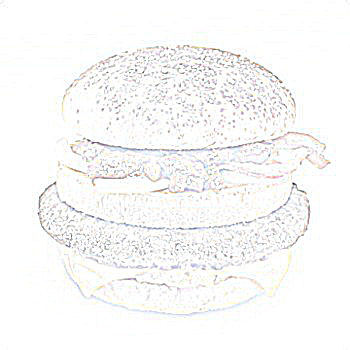
\includegraphics[width=0.45\linewidth]{data/images/theory/theorySift_dog}
%		\captionof{figure}{Example of a Difference of Gaussians with $\sigma=1$ and $\sigma=3$.}
%		\label{fig:dog}
%	\end{minipage}
%\end{figure}

\begin{figure}
	\centering
	\begin{minipage}{.5\textwidth}
		\centering
		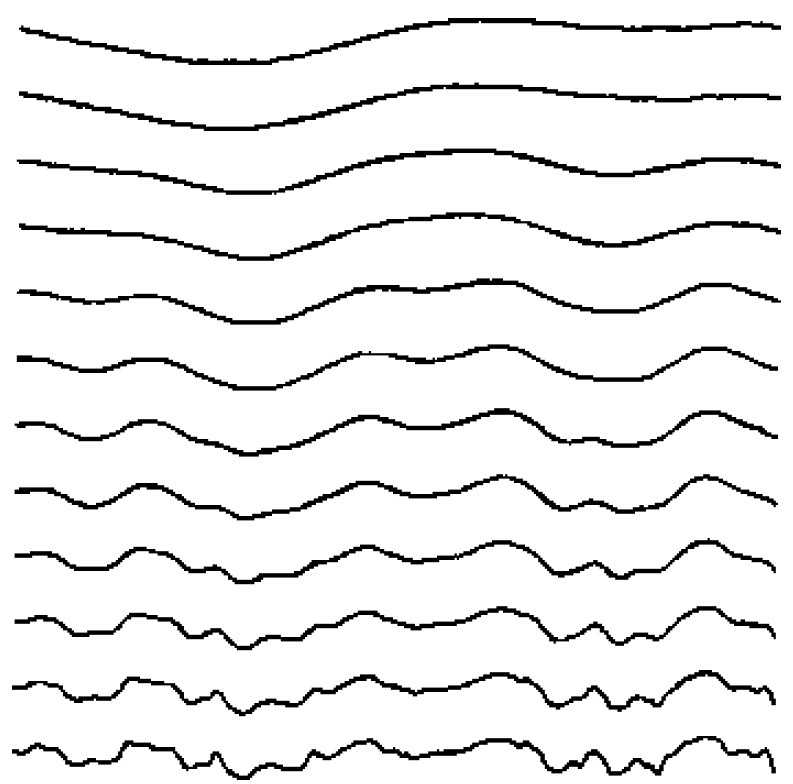
\includegraphics[width=0.45\linewidth]{figures/theorySIFT_scaleSpaceFiltering}
		\captionof{figure}{Sequence of Gaussian smoothings of a 1D graph with $\sigma$ increasing from bottom to top. Source Witkins \cite{Witkin1983}}
		\label{fig:scaleSpaceFiltering}
	\end{minipage}%
	\begin{minipage}{.5\textwidth}
			\centering
			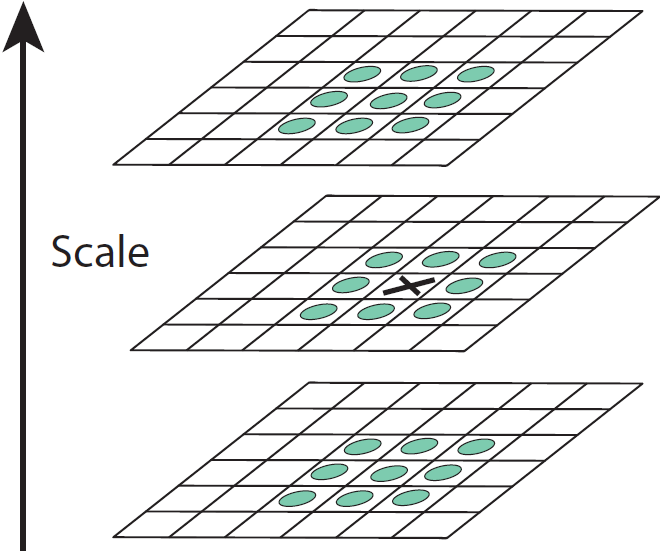
\includegraphics[width=0.45\linewidth]{figures/theorySIFT_interestPointDetection}
			\captionof{figure}{Interest points are detected by searching for minima and maxima. The value of the center pixel {(marked with X)} is compared to its 26 neighbors {(marked with circles)} on the current and adjacent scales. Source: Lowe \cite{Lowe2004}}
			\label{fig:interestPointDetection}
	\end{minipage}	
\end{figure}


The basic idea of \gls{sift}'s keypoint extraction follows Witkins scale-space filtering \cite{Witkin1983}. Witkins found out that by applying Gaussian smoothings at different scales of $\sigma$ on a 1D-graph he could find robust edges depending on the scale of $\sigma$ {(figure \ref{fig:interestPointDetection}a)}. Since this process can also be applied to 2D images scale-space filtering is a good way to find scale invariant interest points {(also called \gls{log})}. \gls{sift}, however, uses a much more computation efficient approximation of \gls{log} called \acrfull{dog} \cite{Lowe2004}. \gls{dog} can be computed by subtracting two adjacent scales from each other. Figure \ref{fig:dogScaleFiltering} shows the process of creating \glspl{dog} at different scales. \gls{sift} samples 3 scales per octave. After each octave the image size is halved and \gls{dog} is applied again on the smaller image {(figure \ref{fig:dogScaleFiltering})}.

\begin{figure}[ht]
	\centering
	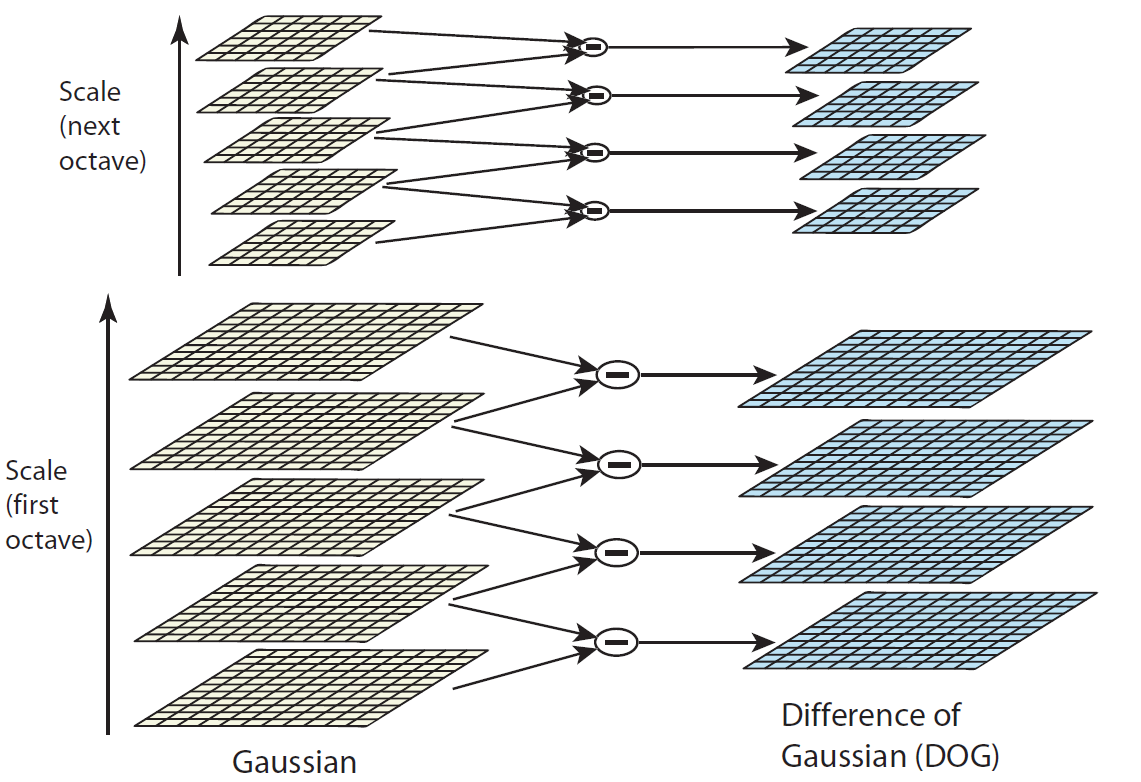
\includegraphics[scale=0.3]{figures/theorySIFT_dogScaleFiltering}
	\caption{For each octaves the image is blurred with Gaussian smoothings at rising scales. A \gls{dog} is formed by subtracting two adjacent scales. After each octave the image size is halved and the process repeated. Source: Lowe \cite{Lowe2004}}
	\label{fig:dogScaleFiltering}
\end{figure}

To check if a pixel qualifies as an interest point at a certain scale, \gls{sift} compares the values of the 3x3 neighboring pixels. If the pixel has the maximum or minimum value \gls{sift} then compares the neighbors on the scales above and below. If the pixel has indeed the lowest or highest value across all 27 points it is taken as a potential interest point {(figure \ref{fig:interestPointDetection})}. The cost of this operation is reasonably low because most of the pixels will be eliminated after the first few comparisons \cite{Lowe2004}. To filter weak interest points, \gls{sift} tries to eliminate low contrast points and points on edges since edges are not very robust features. After the elimination of weak points, \gls{sift} computes a 32-bin gradient orientation histogram in the interest point neighborhood. Orientations are weighted by the magnitude of the gradient. Each bin represents 10\degree of the 360 possible orientations. The bin with the highest peak is then selected as the dominant orientation for this keypoint. Bins with at least 80\% of the highest bin value are selected to form an additional new keypoint.

\subsubsection*{Keypoint Description}
\begin{figure}[ht]
	\centering
	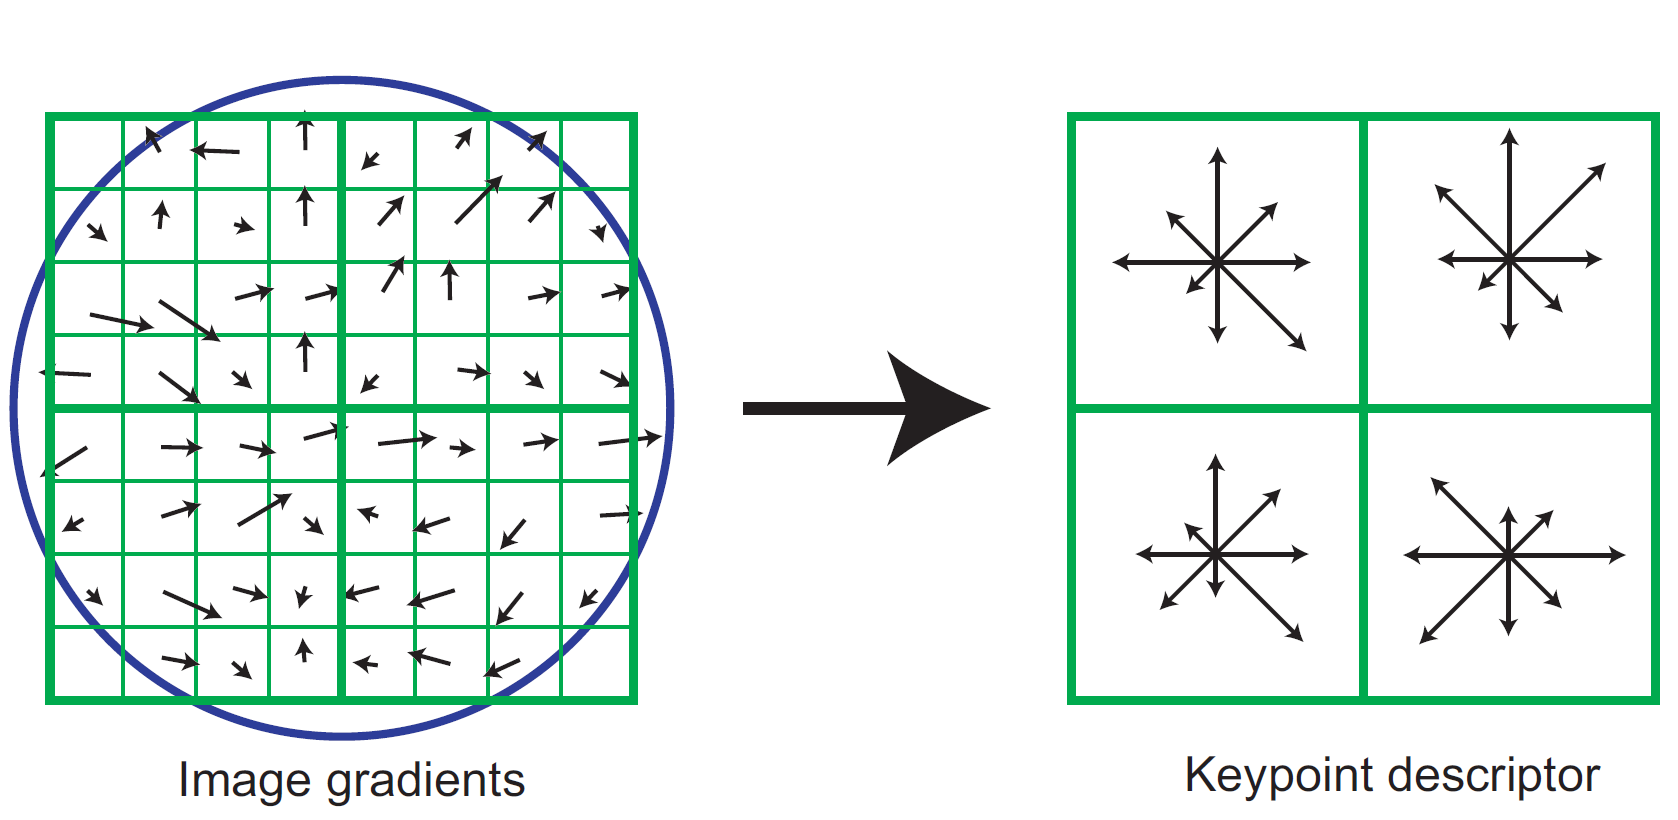
\includegraphics[scale=0.2]{figures/theorySIFT_descriptor}
	\caption{Creation of the \gls{sift} descriptor. Around the keypoint a 16x16 region {(this image is only half the size)} is taken and gradient orientations are calculated. The region forms 16 4x4 blocks with 8-bin gradient histograms. Source Lowe \cite{Lowe2004}}
	\label{fig:siftDescriptor}
\end{figure}
The \gls{sift} keypoint descriptor relies on gradient orientation histograms. They are more stable features than just raw intensity values and less sensitive to 3D rotation. To calculate a descriptor for a keypoint, a neighborhood region of 16x16 pixels is selected oriented along the dominant orientation of the keypoint. The 16x16 region is then divided into 4x4 blocks and for each of these blocks a 8-bin gradient orientation histogram is calculated {(similar to the keypoint extraction)}. This results in a 128 dimensional feature vector for each keypoint {($16\text{ blocks}*8\text{ bins per histogram}=128$)} \cite{Lowe2004}. Figure \ref{fig:siftDescriptor} shows the process of the descriptor creation.

\subsection[SURF]{Speeded up Robust Features (SURF)}
\label{subsec:surf}
\gls{surf} is a feature detector and descriptor which was proposed in 2006 \cite{Bay2006} and later revised in 2008 by Bay et al. \cite{Bay2008}. It was developed with the goal to provide a faster alternative for the popular \gls{sift} algorithm without trade offs in recognition performance.

\subsubsection*{Keypoint detection}
\begin{figure}[ht]
	\centering
	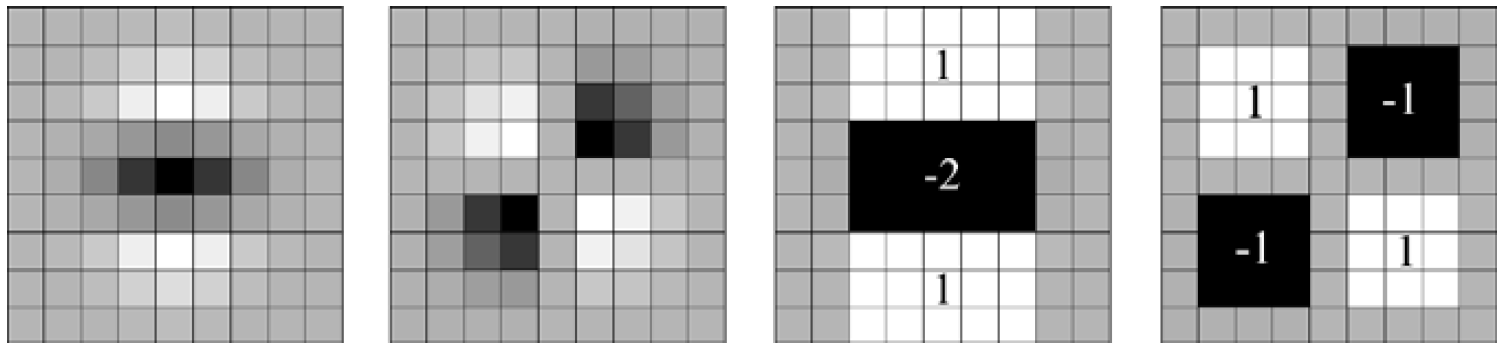
\includegraphics[scale=0.2]{figures/theorySURF_boxFilters}
	\caption{Left half: discretized and cropped Gaussian second order partial derivates in $y$-direction and $xy$-direction. Right half: corresponding box filter approximations. Gray ares are equal to zero. Source Bay et al. \cite{Bay2008}}
	\label{fig:surfBoxFilters}
\end{figure}
Like \gls{sift}, \gls{surf} also uses scale spaces to detect interest points. \gls{surf}, however, relies on an approximation of the Hessian matrix

The first step is to compute the integral image. In integral images, pixel values are the sum of all pixels within a square between the pixel and the origin. These representations are efficient to compute and allow to find the sum of pixel values for any sized box within the image with only four arithmetic operations. Throughout the algorithm this benefit is leveraged to speed up detection and description.

Bay et al. approximate the Hessian matrix using box filters {(in the right of figure \ref{fig:surfBoxFilters})}. By using integral images in combination with box filters the process of scale space creation can be sped up significantly. The benefit of box filters contrary to Gaussians which have to be applied iteratively is, that box filters can be applied directly on the original image which makes parallelization possible. In addition, \gls{surf} does not downscale after each octave. It scales the image up which has the advantage of not causing aliasing. To localize interest points across scales, \gls{surf} applies non-maximal suppression on a 3x3x3 neighborhood. 

\subsubsection*{Keypoint Description}
To achieve rotation invariance, \gls{surf} computes a dominant orientation for each interest point from a circular 6$s$ neighborhood by calculating Haar-wavelet responses in $x$ {(horizontal wavelet response)} and $y$ {(vertical wavelet response)} directions with $s$ being the scale of the interest point. Again, the combination of integral images and wavelets helps to calculate Haar-wavelets efficiently. The dominant orientation is calculated by the use of a sliding rotating window with an angle of $\frac{\pi}{3}$. The wavelet responses are then represented as vectors weighted with a Gaussian of $\sigma=2.5s$. Horizontal and vertical vectors are added and the highest sum is the dominant interest point orientation.

To describe a keypoint, \gls{surf} forms a square neighborhood region oriented along the dominant orientation with a size of 20$s$ {(so keypoints at higher scales include a bigger neighborhood)}. The region is then divided into 4x4 smaller sub-regions. In each of these sub-regions \gls{surf} computes features at 5x5 evenly spaced sample points. Contrary to \gls{sift}, \gls{surf} does not utilize orientation histograms but again Haar-wavelet responses in horizontal $d_x$ and vertical $d_y$ direction relative to the dominant keypoint orientation. $d_x$ and $d_y$ are then summed up over each subregion. Those two and the sum of absolute response values $|d_x|$ and $|d_y|$ form the four dimensional feature vector for each subregion. Therefore, each keypoint has a 64 dimensional feature vector taking into account that there are 16 subregions each with a four dimensional vector. To achieve additional invariance to contrast and illumination changes the feature vector is turned into a unit vector.    

\subsection[ORB]{Oriented FAST and Rotated BRIEF (ORB)}
\gls{orb} is a combination of the corner detection algorithm \gls{fast} \cite{Rosten} and the binary descriptor \gls{brief} \cite{Calonder2010}. \gls{orb} was introduced by Rublee and Bradski in 2011 \cite{Rublee2011} as a replacement for \gls{sift} for low-power devices and real time performance.

\subsubsection*{FAST Keypoint Detection}
\begin{figure}[ht]
	\centering
	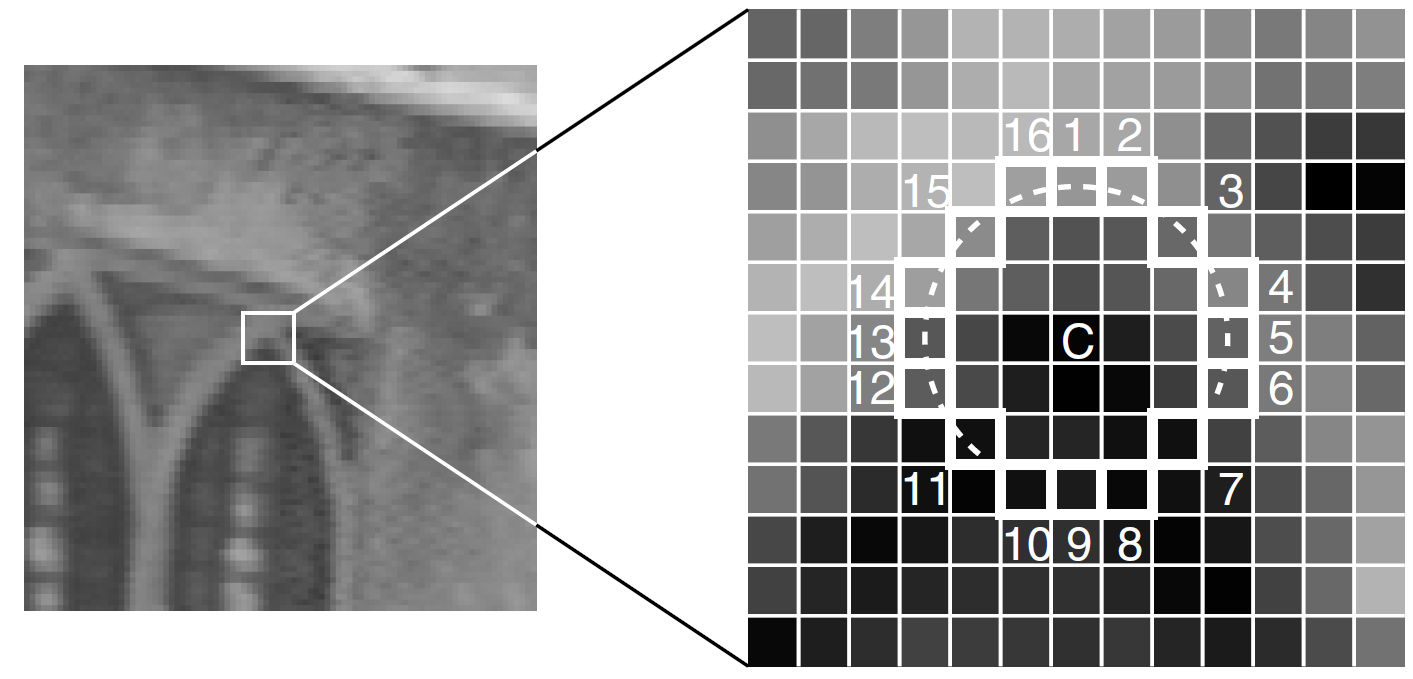
\includegraphics[scale=0.3]{figures/theoryFAST_corners}
	\caption{FAST corner detection. Interest points are selected if at least 12 adjoining pixel values that are either above or below the center pixels intensity {(dashed line)}. Source: Rosten and Drummond \cite{Rosten}.}
	\label{fig:fastCorners}
\end{figure}
\gls{fast} is a corner detection algorithm by Rosten and Drummond from 2006 that does not rely on Gaussians or scale spaces. \gls{fast} compares 16 pixel intensities arranged on a circle with radius 9 around a possible corner point in the center. It is an interest point if it has at least 12 adjoining pixel values that are either above or below the center pixels intensity {(figure \ref{fig:fastCorners})}. \gls{fast}, however, is prone to have many responses along edges which are weaker features so \gls{brief} tries to filter these edge responses by using a Harris corner measure. To achieve scale invariance \gls{brief} applies \gls{fast} on different image pyramid scale spaces. To also make the keypoints rotation invariant, \gls{brief} calculates the intensity centroid which assumes that a corner's maximum intesity is offset from the actual center of the corner. This makes it possible to calculate the orientation by creating the vector from the intensity centroid to the actual corner point.

\subsubsection*{BRIEF Keypoint Description}
\gls{brief} is a binary descriptor from 2010 by Calonder et al. \cite{Calonder2010}. Unlike \gls{sift} or \gls{surf}, a binary descriptor creates the descriptor values by comparing intensity values of pixels in the neighborhood of the keypoint. If the intensity of pixel $a$ is lower than the intensity of pixel $b$ than the test yields "1" and "0" otherwise. To create the feature vector \gls{brief}  performs 256 binary tests and concatenates the results. The pixels that are compared are chosen by a Gaussian distribution around the center of the keypoint. Prior to these tests the image is smoothed. Additional in-plane rotation invariance is achieved by the proposed "steered" \gls{brief}. Steered \gls{brief} rotates the matrix of binary tests by a rotation matrix along the keypoint orientation. A lookup table with precomputed \gls{orb} features is computed with a 12\degree  interval. However, due to the very rotation by steered \gls{brief}, the binary tests loose most of their variance so the expressiveness of the descriptor suffers. To prevent this, Rublee and Bradski proposed an algorithm to "learn" the optimal location of the pixel-pairs that are compared for the binary tests.

\subsection[CenSurE]{Center Surround Extremas (CenSurE)}
\begin{figure}
	\centering
	\includegraphics[scale=0.2]{figures/theoryCenSurE_filters}
	\caption{Center surround filters. From left to right: decreasing accuracy and computational cost.  Source Agrawal et al. \cite{Agrawal2008}}
	\label{fig:censureFilters}
\end{figure}
The \gls{censure} feature detector was proposed by Agrawal et al. in 2008 as a framework of several bi-level filters for interest point detection \cite{Agrawal2008}. \gls{censure} is scale and rotation invariant and similar to the way \gls{sift} and \gls{surf} perform interest point detection. Contrary to the aforementioned keypoint detectors, \gls{censure} does not up- or downscale the image in scale space and therefore does not inherit the disadvantages of up- and downscaling like inaccurate keypoint locations.

To detect corners \gls{censure} employs approximations of \gls{log} with center-surround discrete bi-level filters. The closest approximation of \gls{log} is a circular bi-level filter as shown in figure \ref{fig:censureFilters}a. Bi-level means that the filter only contains two values namely $1$ or $-1$. The circular filter is rotation invariant due to its symmetry but it is also expensive to compute. Therefore, \gls{censure} uses octagons and boxes as approximations of the circular filter. Like \gls{surf}, \gls{censure} also leverages integral images for box filters and applies them on five scales. Since a major shortcoming of box filters is the lack of rotation invariance Agrawal et al. also proposed an octagon shaped filter which resembles the circle filter much more closely. Integral images, however, do not work with diagonal edges and thus do not work with octagons. To make computation still possible Agrawal et al. introduced "slanted" integral images which are able to construct any trapezoidal area in the same amount of time as rectangular integral images. 

To detect interest points, \gls{censure} performs non-maximal suppression over scale space across a 3x3x3 neighborhood. Weak interest points are filtered by threshold and edges are filtered the Harris corner measure.

\section{Bag of Words}
\acrfull{bow}, bag of features, bag of visual words or bag of keypoints is a simple, yet powerful image feature quantization method. The original idea of a \gls{bow} approach for images came from texture classification \cite{Leung2001}. Leung and Malik found out that by quantification of small texture patches {(textons)} in histograms they were able to accurately classify different textures. In 2004 Csurka et al. refined this approach and applied it to general image classification \cite{Csurka2004}.

The idea behind a \gls{bow} is very simple: During learning the \gls{bow} clusters image descriptors using $k$-means clustering. The clustered representation of the image descriptors is called vocabulary. The vocabulary size is $k$, so using $k=1000$ for the k-means clustering results in a vocabulary of 1000 image features. Choosing $k$ is a trade-off between speed and accuracy and has to be determined during experiments. In an ideal world, a \gls{bow} clusters image features together that are unique and expressive so that we would have a vocabulary of bread, salad, meat and noodle features.

During classification the \gls{bow} gets a set of image descriptors and matches these features with the previously learned vocabulary. The output of this process is a histogram of vocabulary occurrences. Referring to the ideal world example, the \gls{bow} would get a set of features including many that look like bread, some that look like meat and a few that are similar to the salad texton. The output would be a histogram with a large value for the bread bin and some smaller values for the salad and meat bins. Giving this occurrence vector to a trained SVM would reveal that the image might be a Hamburger.


\section{Methodology}
\subsection{Performance Measurements}

\subsubsection*{Precession - Recall}
The most used measure for the precision of food classifiers is the average accuracy which is calculated by dividing the number of correct matches and the total number of samples. Accuracy, however, gives no information about the underlying conditions. It is a measure of overall performance. To have a higher chance of suggesting the correct items, future systems may present a list of options that the user can chose from. Intuitively, the accuracy is much higher if a classifier can present a list of items with high confidences instead of only one item because the problem is much easier. Accuracy, however, does not measures how easy a problem is. If a classifier were able to suggest all classes as options the accuracy would always be 100\% although the results are not useful at all.

The combination of precision and recall objectively measures the actual relevance and performance of a classifier for a class of images because it includes the amount of considered items and the correct predictions. In this case the amount of considered items changes based on how many items the classifier can suggest. Precision and recall is defined as:

\begin{equation}
Precision = \frac{T_p}{T_p+F_p} \quad Recall = \frac{T_p}{T_p+F_n}.
\end{equation}

\begin{itemize}
	\item True positives $T_P$ is the number of correctly classified images of a class.
	\item False positives $F_P$ are all images that the classifier predicted to be positive but are in reality negative. {(Type I Error)}
	\item False negatives $F_N$ are all images that are positive {(belong to the class)} but are labeled as negative {(do not belong to class)} {(Type II Error)}
\end{itemize}

A high recall means that many images were matched correctly and a high precision denotes a low number of incorrectly classified images. The bigger the area under the Precision-Recall curve the better the classifier.

\subsubsection*{Null Error Rate}
The null error rate is a baseline for any classification task that calculates the accuracy if a classifier would just predict the class with the most images.

\subsubsection*{Confusion Matrix}
Confusion matrices are one of the most important metrics to understand why a classifier struggles with certain classes while getting a high precision with others. As the name suggests, a confusion matrix tells if the classifier "confuses" two classes.

A confusion matrix for $n$ classes is always a $n \times n$ matrix where columns represent the actual images classes and rows represent the predicted image classes so if the diagonal of the matrix has high values this means that the classifier makes correct predictions.

\subsubsection*{Categorical Cross-Entropy}
The categorical cross-entropy $L_i$ is an error function that is used for the training of neural networks in classification tasks as the objective function. It is more versatile than the accuracy or the \gls{mse} because it takes the deviations of the predicted label $p_{i,j}$ and the actual label $t_{i,j}$ into account and weights the "closeness" of the prediction with the logarithm. For classification, cross entropy is more useful than \gls{mse} because \gls{mse} gives too much emphasis on incorrect predictions. The categorical cross entropy function is defined as:

\begin{equation}
L_i = - \sum_{j} t_{i,j}\log(p_{i,j})
\end{equation} 

The loss values that are used for the discussion of results for neural networks are the average values of the categorical cross-entropy {(\gls{ace})}.

\subsection{Cross Validation}
Cross validation is one of the most essential techniques to evaluate real-world classification performance. Classifiers like \glspl{svm} or neural networks are always better on data they have already seen. This is called overfitting {(see section \ref{subsec:overfittingDropout})}. By training and testing on the same data the classification performance would be much better than the actual real world performance. To test if a classifier can actually work with samples it has not seen cross validation divides the dataset into different partitions. 

For most tasks it is sufficient to divide the dataset into a training and a test set. The data in the training set is used to train the classifier and the test data is used to evaluate it with data is has not seen before.

\subsubsection*{k-fold Cross Validation}
To make the classification evaluation even more robust, $k$-fold cross validation is used. By applying $k$-fold cross validation the dataset is randomly partitioned into $k$ different parts. $k-2$ parts are used for training and two parts are used for the evaluation. This process is repeated $k$-times and after each iteration the parts are exchanged so that at the end, each sample was used for training and for validation. Calculating the mean of the $k$ evaluations gives a much more robust measurement because the evaluation does not depend on the difficulty of the test partitions.
